\chapter{Methodology}
    \label{chap:methodology}
    
In this chapter, we will be discussing the research methodology of the project, then explain the implementation of the proposed model and the metrics which will be used in experiments.

As you will see later in section \ref{sec:proposed_model}, our proposed model is a combination of the methods of \cite{athalye} and \cite{zheng_black_box_GAN}, and therefore it is necessary to implement those papers and re-create some of the results of those papers to ensure these implementations are correct, before merging the two for our own model. Therefore, we will cover these implementations in sections \ref{sec:eot_implementation} and \ref{sec:zheng_implementation}.
    
\section{Research methodology}

The EOT framework presented in subsection \ref{subsec:eot} is highly effective at creating robust adversarial noise for 3D-rendered objects. This is despite the fact it is training on renders of the object with a random position and angle. In EOT, the transformation from the texture to the rendered image is represented as a simple linear transformation. At the same time, generative models have proven to be capable at learning a distribution for generating large 256x256 images \cite{big_gan}, especially benefiting from having significantly more parameters. Therefore, my intuition is that with the proper training hyper-parameters and architecture, a generative model should be able to learn to create adversarial textures. Since the transformation representing 3D rendering is linear, it should not be an insurmountable obstacle for training the generator.

Moreover, the black-box generative model in subsection \ref{subsubsec:zheng} can be easily combined with the EOT framework for making adversarial objects in subsection \ref{subsec:eot}, by placing a differentiable rendering pipeline between the generator and the simulator.

\newpage
The research hypothesis of this project is the following: 

\textit{It is possible to use a generative neural network to create 3D-rendered adversarial objects in the targeted black-box setting that have a targeted fooling rate of at least 50\% on a victim CNN classifier for object recognition.}

\bigbreak
The targeted fooling rate metric is explained later in section \ref{sec:analytic_techniques}.

This is a quantitative experimental research project. The model proposed in section \ref{sec:proposed_model} creates 3D-rendered objects, and pictures of those objects will be given to various neural network classifiers. The predicted label will be compared against the correct label and the adversarial target label to evaluate the effectiveness of the proposed method. We will mainly be using a circulatory research process, to try Further details on the experiments are found in subsection \ref{sec:experiment_design}.

\section{Implementation of EOT}
    \label{sec:eot_implementation}

Like subsection \ref{subsec:eot} mentioned, the authors of \cite{athalye} fail to include detailed information into how they represented 3D rendering as a differentiable linear transformation. One of the authors provides a step-by-step guide with source code \cite{athalye_step_by_step}, but only for attacks for 2D images, not for textures which are then rendered as 3D objects. I therefore searched Github.com for repositories related to \cite{athalye}, and found one implementation of the paper for the 3D rendered objects case \cite{ring_adversarial_3d}. 

However, the implementation lacked documentation and was written in Tensorflow 1, which is obsolete, less intuitive and harder to debug. I forked the repository and almost completely re-wrote the code to run with Tensorflow 2 \footnote{Source code at https://github.com/Alexandru-Dascalu/adversarial-3d}, documented it and refactored it according to software engineering principles, although the algorithm is broadly the same as \cite{ring_adversarial_3d} implemented it.

\subsection{UV mapping}

3D models are made up of a series of vertices, points in 3D space which define the shape of an object. To apply a texture to a model, one method is to use UV coordinates, which are pairs of coordinates which tell you which pixel from the texture image should be used to colour a certain vertex. These coordinates are defined when the 3D model is created, and come included with the vertex coordinates in the 3D model file. After rendering a 3D model, an OpenGL renderer will look up the UV coordinates for each vertex, and for each triangle it will copy the fragment of the texture that is within the three texture coordinates of the triangle, thus creating a textured object. A UV map is what Athalye \textit{et al.} \cite{athalye} likely referred to when talking about texture-space coordinates.

A normal renderer will take the array of vertices, the UV map and the object's texture as inputs. It will first render the object by translating and rotating the position vector of each vertex \cite{opengl_shaders}. Following that, it will use the UV coordinates of each vertex to sample a colour from the texture, either by using nearest-neighbour, bilinear interpolation or anisotropic filtering \cite{opengl_textures}. However, the renderer implemented by \cite{ring_adversarial_3d} and used by us simply returns the UV coordinates instead of a colour. Therefore, the output of the renderer is a 299x299 image of the object rendered in the desired pose, but instead of a colour with RGB values, each pixel has a U and V coordinate pointing to a pixel in the texture. We are going to call this output image a "UV map" from now on.

The renderer is implemented using ModernGL \footnote{https://github.com/moderngl/moderngl}, a Python wrapper around OpenGL which allows you to render .obj files with textures.

\subsection{Transformation from texture to image}
    \label{subsec:eot_transformation}
    
\begin{algorithm}
\caption{Pseudo-code representation of the transformation function $t(\cdot)$}
\label{alg:rendering}
\begin{algorithmic}[1]
\STATE $std\_textures \gets repeat(std\_texture)$
\STATE $adv\_textures \gets repeat(adv\_texture)$
\IF{print\_error}
    \STATE $std\_textures, adv\_textures \gets apply\_print\_error(std\_textures, adv\_textures)$
\ENDIF
\STATE $std\_image \gets resample(std\_textures, uv\_maps)$
\STATE $adv\_images \gets resample(adv\_textures, uv\_maps)$

\STATE $std\_images, adv\_images \gets add\_background(std\_textures, adv\_textures)$

\IF{photo\_error}
    \STATE $std\_images, adv\_images \gets apply\_photo\_error(std\_images, adv\_images)$
\ENDIF

\STATE $std\_images, adv\_images \gets normalise(std\_images, adv\_images)$
\RETURN $std\_images, adv\_images$
\end{algorithmic}
\end{algorithm}

The renderer produces a UV map for each image in the mini-batch, which together with the texture is used as input for the algorithm seen in algorithm \ref{alg:rendering}. This algorithm is a step-by-step representation of the $t(x) = Mx + b$ function mentioned in section \ref{subsubsec:eot_technique}. As we will see, this algorithm is indeed just a linear transformation. The reason that this algorithm creates images with both the original and adversarial paper is that we need to calculate difference between them for the penalty term in equation \ref{eq:eot} on page \pageref{eq:eot}. Since this penalty seeks to measure the perceptual difference caused by the adversarial noise, all other parameters such as the pose of the object or the background colour must identical for each pair made up of a normal and an adversarial image.

The $repeat(\cdot)$ function in lines 1 and 2 of the pseudocode simply replicates the 3D texture tensor as many times as the size of the batch, as you can see in listing \ref{lst:repeat}.

\lstinputlisting[language={python}, label={lst:repeat}, caption={An implementation of the repeat function from algorithm \ref{alg:rendering}}]{./listings/repeat.py}

\lstinputlisting[language={python}, label={lst:print_error}, caption={Simulating 3D printer errors.}]{./listings/print_error.py}

Athalye \textit{et al.} \cite{athalye} modelled per-colour channel 3D printer errors in their experiments with 3D-printed adversarial objects. The $apply\_print\_error$ function implements this by randomly generating a scalar multiplier and addend for each colour channel in each batch texture, and using those to linearly transform the texture, as you can see in listing \ref{lst:print_error}.

After applying the print error, we can create the batch of 299x299 images of the rendered object. The $resample(\cdot, \cdot)$ function from algorithm \ref{alg:rendering} is implemented as the $resampler(\cdot, \cdot)$ method from the tensorflow\_addons library \cite{tfa_resampler}. For each pixel in each image, it samples a colour from that image's texture based on the UV coordinates of the corresponding pixel in that image's UV map. tensorflow\_addons.resampler uses bilinear interpolation to mix the colours of neighbouring texture pixels to get the colour it will return \cite{tfa_resampler}. Therefore, it is a linear transformation.

\lstinputlisting[language={python}, label={lst:add_background}, caption={Code for adding colour background to the renders of the 3D object.}]{./listings/background.py}

In \cite{athalye}, the authors used random colours for the background of each render. Therefore, for each image we compute a mask with true boolean values for each pixel that makes up the object. The UV maps have a value of 0 for each pixel that makes up the background of the scene rather than the object, so we just check for UV coordinates different than 0. We then sample an RGB colour from a truncated uniform distribution. We obtain the background by performing element-wise multiplication between the colour vector and a logical inverse of the mask, which has true values for the background and false for the object. We then add that with a multiplication between each image with its mask, which essentially "cuts out" the rendered object and adds it on top of the background. This process can be seen in code listing \ref{lst:add_background}.

Since a 3D-printed adversarial object would be photographed with a camera connected to a neural network, Athalye \textit{et al.} \cite{athalye} also modelled random lighting conditions and camera noise in their experiments with physical objects. Our implementation, represented by the $apply\_photo\_error(\cdot, \cdot)$ function in algorithm \ref{alg:rendering}, linearly scales each image with a random scalar multiplier and addend to lighten or darken the image. It then simulates camera noise by adding gaussian noise.

\lstinputlisting[language={python}, label={lst:normalise}, caption={Source code for normalising the rendered images}]{./listings/normalise.py}

Finally, the $normalise(\cdot, \cdot)$ function from algorithm \ref{alg:rendering} linearly normalises the images, as the random scaling done when applying the photo or print error may result in values outside $[0, 1]$. Firstly, we calculate the minimum and maximum pixel values across all colour channels for each image. We will then pick the minimum and maximum values for each pair of normal and adversarial images. This is important, as the adversarial noise may fall outside $[0, 1]$, and because it is semantically meaningful, the normal image must use the linear scale as its adversarial counterpart. Finally, if a minimum or maximum value is inside $[0, 1]$, we set it to 0 or 1, respectively. This is because scaling is done only to bring invalid values inside the valid range. This normalisation process can be seen in code listing \ref{lst:normalise}.

\subsection{Creating the adversarial texture}

The rest of the implementation works just how subsection \ref{subsubsec:eot_technique} described the EOT framework \cite{athalye}. Rendered images of the 3D model are created using the algorithm described in subsection \ref{subsec:eot_transformation}. As seen in the code listings in subsection \ref{subsec:eot_transformation}, these renders are dependent on parameters drawn from uniform distributions for the rotation, camera distance, X/Y translation, print error, lighting, camera noise and background colour.

The rendered images are given to the victim model for inference. The resulting logits, together with the target labels, are used to calculate the average cross-entropy loss across all images in the mini-batch. This is the first term of the objective function in equation \ref{eq:eot} on page \pageref{eq:eot}. Furthermore, we calculate the second term of that equation by projecting the normal and adversarial images into LAB space \cite{lab} using the scikit-image library \footnote{https://scikit-image.org/docs/dev/api/skimage.color.html\#skimage.color.rgb2lab}, then calculating the average $\ell_2$ norm of the difference between each of pair of normal and adversarial images. An Adam optimiser is used to update the adversarial texture such that the objective function in equation \ref{eq:eot} is minimised.

At each optimisation step, a certain percentage of rendered images from the previous mini-batch are re-used, as Athalye \textit{et al.} also did. This is implemented by shifting the previous tensor of images to the left, thus discarding some of the images from the previous mini-batch, then adding the new renders at the end. Therefore, old renders are gradually replaced. For example, with a re-use percentage of 80\%, there is an entirely new batch of renders after every 5 optimisation steps. For added efficiency, the logits of the victim model for old renders are memorised rather than re-calculated at each stop, logits are computed only for the new renders.

\section{Implementation of Zheng et al.'s model}
    \label{sec:zheng_implementation}
    
I searched Github.com for an existing implementation of Zheng \textit{et al.} \cite{zheng_black_box_GAN}, and found a Tensorflow implementation made by the authors of the paper themselves \footnote{https://github.com/StanleyZheng-FDU/targeted-black-box-attack}. Unfortunately, it was also written in Tensorflow 1, lacked documentation and had a lot of duplicate or unused code. On the other hand, it implemented all models and training techniques described by Zheng \textit{et al.} \cite{zheng_black_box_GAN}.

Due to time constraints, I chose not to completely re-write this implementation in Tensorflow 2. I forked the repository \footnote{https://github.com/Alexandru-Dascalu/targeted-black-box-attack} and only added some comments, some minor refactors to improve code readability and some code to plot the training history.

\section{Proposed model for G-EOT}
    \label{sec:proposed_model}
    
\subsection{Overview}
    \label{subsec:g_eot_overview}

The proposed G-EOT model is at a high level the same generative model presented in subsection \ref{subsubsec:zheng}, except that it has elements of the EOT framework \cite{athalye} added to it. The key difference is that the generator produces adversarial perturbations for a 2D texture rather than an image of an object, as you can see in figure \ref{fig:architecture}. The perturbations are then added to the original texture to create the adversarial texture. The latter is then rendered as a 3D object, and an image of the rendered object is then given to the simulator and to the victim model.

\begin{figure}[h]
    \centering
    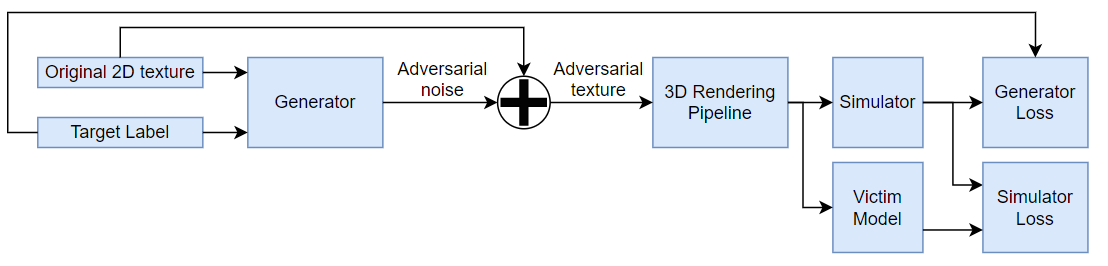
\includegraphics[width=1\textwidth]{graphics/architecture.PNG}
    \caption{The architecture of G-EOT.}
    \label{fig:architecture}
\end{figure}

The 3D rendering pipeline in figure \ref{fig:architecture} is essentially identical to the one presented in section \ref{sec:eot_implementation}. It simulates 3D rotation, translation, varying camera distance, different background colours and lighting conditions, camera noise, and 3D printer error. The parameters for 3D rendering are sampled from truncated uniform distributions, similarly to the distribution $T$ of transformation functions presented in the supplementary material of \cite{athalye}. 

All textures for 3D models that I could find had at least 1024x1024 pixels, with most having a resolution of 2048x2048. Since generative models struggle to generate output larger than 256x256 pixels \cite{big_gan}, the generator first performs average pooling on the texture to reduce its resolution. The adversarial noise created by the generator has a resolution of 256x256. This is then upsampled using bilinear interpolation to 2048x2048 pixels so that it can be added to the original texture to obtain the adversarial texture.

\begin{wrapfigure}[27]{r}{0.3\textwidth}
    \centering
    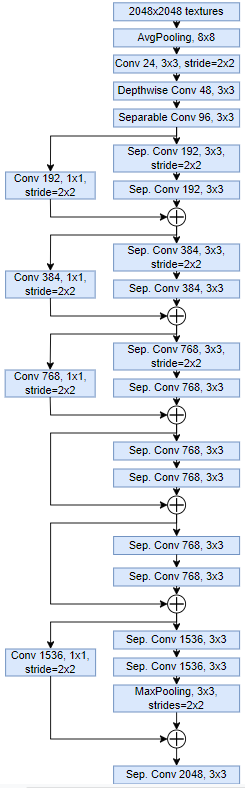
\includegraphics[width=0.3\textwidth]{graphics/g_eot_encoder.PNG}
    \caption{The structure of the encoder in the G-EOT generator.}
    \label{fig:proposed_encoder}
\end{wrapfigure}

EOT \cite{athalye} was chosen rather than $\textrm{RP}_2$ \cite{evtimov_road_signs} because it is a lot more convenient, for reasons named in subsection \ref{subsubsec:rp2_results}. Furthermore, the synthetic transformation functions for 3D rendered objects can accurately simulate real-world transformations \cite{athalye}. On the other hand, the method presented in Zheng \textit{et al.} \cite{zheng_black_box_GAN} was chosen for the genera-simulator model rather than one from Xiao \textit{et al.} \cite{advGAN} because it is simpler and it can generate attacks for all target labels, as mentioned in subsection \ref{subsec:AdvGAN}.

\subsection{Generator}

The generator is an auto-encoder with a similar structure as the one in figure \ref{fig:zheng_generator} in subsection \ref{subsubsec:zheng}. Its encoder is a CNN with an architecture inspired by the SimpleNet CNN from Zheng \textit{et al.} \cite{zheng_black_box_GAN}, which is itself inspired by Xception \cite{xception}. 

Its structure can be seen in figure \ref{fig:proposed_encoder}. The numbers after the type of the convolutional layer are the number of output channels of that layers, followed by the kernel size. Although not seen in the diagram, each convolutional layer is followed by a batch normalisation layer \cite{batch_norm}.

Meanwhile, the structure of the decoder is exactly the same as the one in Zheng \textit{et al.} \cite{zheng_black_box_GAN}, shown in figure \ref{fig:zheng_decoder} on page \pageref{fig:zheng_decoder}. A more detailed diagram of the generator is in appendix \ref{app:detailed_architecture}.

The loss function used to train the generator is the same as equation \ref{eq:generator_loss} on page \pageref{eq:generator_loss} describes, except that it is not enough for the penalty term to be the $\ell_2$ norm of the adversarial noise, as the victim model does not perceive the texture directly, but rendered images of the 3D model instead. Therefore, the penalty term used is:

\begin{equation}
    \label{eq:g-eot-l2-loss}
    \begin{aligned}
    \beta\|t(x + G(x,z)) - t(x)\|_2
    \end{aligned}
\end{equation}

\noindent where $x$ is the original texture, $z$ is the target label, $t(\cdot)$ is the transformation function represented by the 3D rendering pipeline, and $G(\cdot, \cdot)$ is the adversarial noise created by the generator. The image with the adversarial texture and the image with the normal texture use the same function $t(\cdot)$ so that the images will have the same pose, and the only difference is caused by the perceived adversarial noise. I chose not to project the images into LAB space, as Athalye \textit{et al.} did, to simplify the training task of the generator.

\subsection{Simulator}

\begin{wrapfigure}[24]{r}{0.3\textwidth}
    \centering
    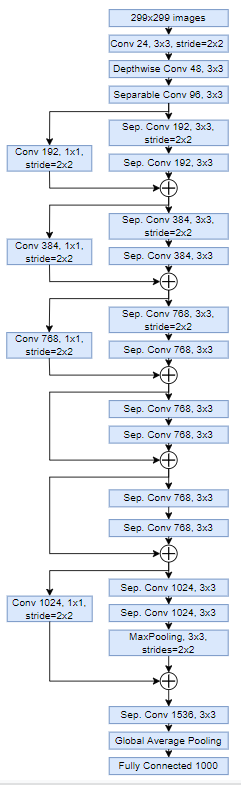
\includegraphics[width=0.3\textwidth]{graphics/g_eot_simulator.PNG}
    \caption{The structure of the G-EOT simulator.}
    \label{fig:proposed_simulator}
\end{wrapfigure}

The simulator is also a CNN inspired by the SimpleNet architecture from Zheng \textit{et al.} \cite{zheng_black_box_GAN}, and it is almost identical to the architecture of the encoder, though its last three convolutional layers have fewer kernels, and it has a global average pooling and a fully connected layer at the end, and it does not have the average pooling layer at the beginning. It can be seen in figure \ref{fig:proposed_simulator}, and a more detailed diagram is in appendix \ref{app:detailed_architecture}.

Moreover, the loss function for training the simulator is the same as equation \ref{eq:simulator_loss} from subsection \ref{subsubsec:zheng}. 

\subsection{Training techniques}
    \label{subsec:training}

Firstly, the simulator is warmed up by training it to predict the same labels as the victim model does on images rendered using normal textures. This is done to speed-up training, as Zheng \textit{et al.} \cite{zheng_black_box_GAN} explained.

Following that, the simulator and generator are trained in alternative steps. In each simulator training steps, two steps are actually performed to train the simulator to imitate the victim model. In the first one, the simulator and victim model are given as input images rendered with normal textures. In the second one, they are given images with textures perturbed by the generator. This is done to ensure that throughout training, the simulator further learns to be an accurate imitation of the black-box victim model.

Then a training step is performed for the generator. It trains to generate adversarial noise for textures such that images rendered with those textures fool the simulator, as described by equation \ref{eq:generator_loss} in subsection \ref{subsubsec:zheng} and in subsection \ref{subsec:g_eot_overview}. The gradients of the generator loss function are clipped before they are applied, just as Zheng \textit{et al.} \cite{zheng_black_box_GAN} did for their model.

Unlike in Athalye \textit{et al.} \cite{athalye}, no renders are re-used between mini-batches. This is done because it has been observed that the maximum batch size for G-EOT that can fit in 8GB of memory is only 5. Generating 5 new renders for each training step can be done fast enough, and the model trains better the more new unique samples it sees.

\section{Analytic techniques}
    \label{sec:analytic_techniques}
    
Unless otherwise specified, each experiment will use the following metrics to evaluate the proposed attack's success:

\begin{itemize}
    \item \textbf{Targeted Fooling Rate (TFR):} the percentage of adversarial examples that are classified by the victim model as the desired target label. Please note that TFR is the same thing as the adversariality metric used in Athalye \textit{et al.} \cite{athalye}. It is also frequently called "attack success rate" in the literature.
    \item \textbf{Untargeted Fooling Rate (UFR):} the percentage of adversarial examples that are classified by the victim model as any incorrect label. It is relevant because if the attack induces a misclassification, even if it is not the desired target label, then it is still potentially dangerous.  It is always equal to $1 - accuracy$.
    \item \textbf{Classification Accuracy:} the percentage of adversarial examples classified with the correct label. It is always equal to $1 - UFR$.
\end{itemize}
